To estimate the impact of beaver reintroduction on agricultural land use, I obtain data on (1) the Tayside beaver expansion from three comprehensive regional surveys conducted over a decade, (2) high-resolution satellite-derived land use classifications, (3) soil data on agricultural land compatibility, (4) river level from a network of in-situ hydrometry monitors across Scotland, and (5) annual weather patterns. To measure the impacts of beaver entry on agriculture, I employ the land use data, exploiting its spatiotemporal variation, spanning pre- and post-beaver entry periods, to test for land use change. To detect physical environment changes following beaver entry, I use the hydrometry data. In robustness checks, I use high-resolution data on soil type, elevation, and slope to run models on subsamples varying beaver habitat suitability. In all analyses, the unit of observation is a 1km$^2$ cell in a grid constructed by tessellating the study region in Fig. \ref{fig:study-area}. Subsamples of only ``river'' cells rely on a watercourse layer sourced from Ordnance Survey OpenData (CITE?).

\subsection{Beaver Expansion}
Beavers reemerged in Scotland after 2000 around the River Tay, with anecdotal reports beginning around the middle of the decade and NatureScot, Scotland's national conservancy, acknowledging their presence in 2006. In 2012, NatureScot conducted the first comprehensive survey of beaver presence (\cite{campbell_rd_naturescot_2012}). Two follow-up surveys were conducted in 2017-18 and 2020-21, respectively, with each resurveying the extent of its predecessor as well as extensions along suitable habitat corridors. The surveys were carried out in canoe and on foot, with the 2012 survey covering 690km of contiguous watercourse and 450km of non-contiguous river bank around the rivers Tay, Tummel, Isla, Almond, and Earn.\footnote{An additional 310 km of river bank had been surveyed over several preceding years, informing the initial targets of the 2012 survey.} The 2020-21 survey covered 1,760km of contiguous watercourse, 1,238 non-contiguous spot checks along river banks (\cite{campbell-palmer_r_naturescot_2021}). Of the 1,522 field signs recorded in 2012, most were cutting, with only six direct beaver sightings. 98\% of field signs were found within 10m of a watercourse. I obtain beaver survey records via the National Biodiversity Network Trust's NBN Atlas repository, which contains a limited number of the variables recorded by surveyors. In data aggregation, I focus solely on the extensive margin of beaver expansion for several reasons. First, data sharing privacy constraints did not allow for collection of the full set of variables needed to estimate beaver population.\footnote{These include activity type (e.g., dam, foraging, scent mound), estimated age, distance from water, effected area, and river width/depth, among others.} Second, a change in GPS data collection methods in the 2017-18 survey inflated the number of observations linked to any given field sign, a discrepancy for which the full set of variables would be needed to adjust (\cite{campbell-palmer_r_naturescot_2018}). Finally, because much of the survey work was conducted during summer months, vegetation cover obscured many beaver signs, making precise quantification unreliable.

Over the decade of surveys, beaver populations expanded rapidly, more than doubling between each survey despite both official and unauthorized control operations. The 2012 survey detected 39 beaver groups in the Tayside region. In 2018, this had risen to 114 groups. In 2021, 251 groups were found (\cite{campbell-palmer_r_naturescot_2021}). Fig. \ref{fig:beaver-expansion} shows beaver expansion throughout the tessellated study region. Grid cells are colored according to the first year in which a NatureScot survey detected any beaver sign. The observed pattern accords with ecological literature on beaver colonization. Dispersal occurs linearly along waterways, both downstream and upstream (\cite{muller-schwarze_beaver_2011}), with separate groups initially far apart to avoid territorial conflict, then slowly filling over time (\cite{hartman_patterns_1995}).

\begin{figure}
    \centering
    \caption{Beaver Expansion}
    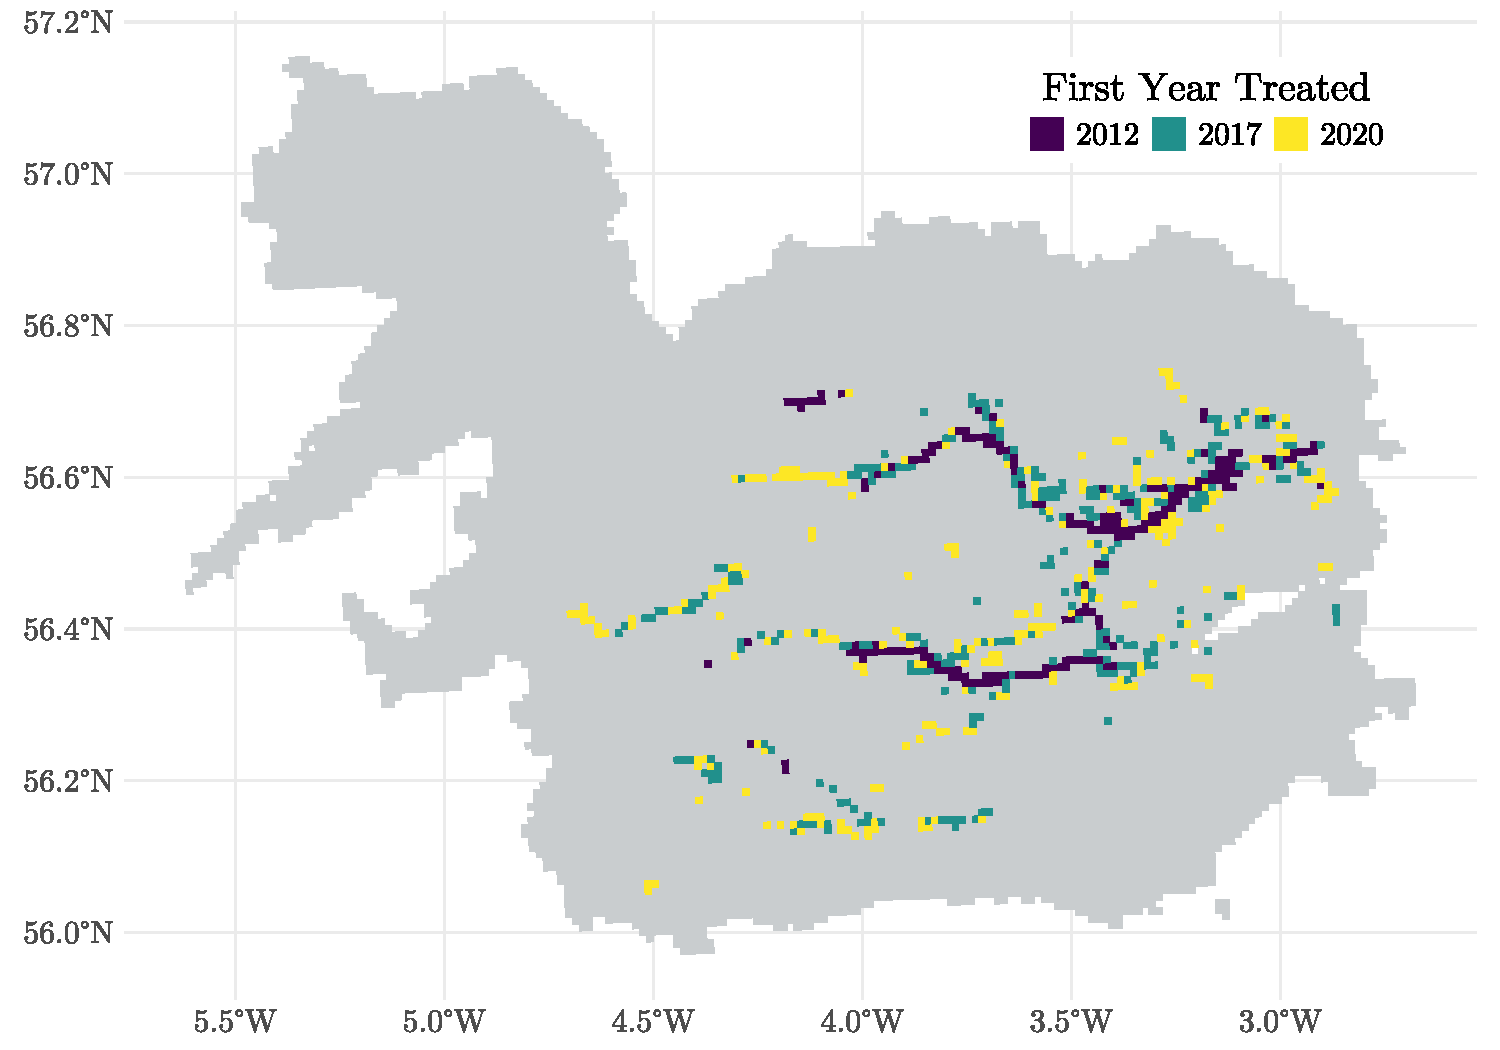
\includegraphics[width=0.7\linewidth]{output/figures/beaver_first_year_treated.pdf}
    \label{fig:beaver-expansion}
    \caption*{\justifying \footnotesize Notes: Beaver detection by survey year in study region. Observation units are 1km$^2$ landscape grid cells. Data source: NatureScot and affiliated survey contractors. See main text for details.}
\end{figure}

\subsection{Land Use}
To capture spatiotemporal variation in agricultural land use, I employ the UK Center for Ecology \& Hydrology's repeated Land Cover Map product (LCM) at 25m resolution, which exists for 1990, 2000, 2007, 2015, 2017, 2018, 2019, 2020, 2021, and 2022. The LCM covers the entirety of Great Britain and North Ireland, deriving its classifications from Sentinel-2 10-band seasonal composite image patches\footnote{Sentinel-2 was launched in 2015. 1990-2015 maps used Landsat 30m resolution imagery. In 2017, UKCEH revised its historical classifications to allow for comparability with post-2015 products.}, with additional context layers on height, aspect, slope, distance to built structures and water bodies, foreshore, and woodland to ejudicate spectral confusion \citep{noauthor_ukceh_2024}. Modern UKCEH models (since 2015) classify 10m pixels into 21 land use classes, based on the Biodiversity Action Plan Broad Habitats \citep{jackson_guidance_2000}, using a random forest. As ground truth, UKCEH uses pixels classified in previous years with high accuracy (>80\%) and no observed change over three consecutive years. Predictions made on 10m pixels are then aggregated to land parcels and from there rasterized at 25m resolution. I consider agricultural any pixel classified as ``arable'' in the UKCEH LCM, which includes cropped and freshly ploughed land (Fig. \ref{fig:ukceh-lcm-raw}). I do not include the closely related class of ``improved grassland'' due to its low recall and precision (74.3\% and 91.1\%, respectively) compared to ``arable,'' which has the highest recall and second highest precision of any class (97.6\% and 92.7\%, respectively), when validated on a set of reference points sourced from countryside surveys, National Forest Inventory, Rural Payment Agency, manual Sentinel-2 image interpretation, and UKCEH field collection.\footnote{This is largely due to the difficulty of differentiating between grassland types, including improved, neutral, calcareous, and acid, which exist on a spectral continuum.} Nearly all false negative arable pixels were mislabeled as improved grassland (93.4\%). Similarly, the majority of false positive arable-classified pixels were in fact improved grassland (55.8\%). I aggregate the 25m ``arable'' mask up to the 1km$^2$ grid cells to produce a measure on the unit interval of agricultural land share, weighting by overlap proportion for raster cells not entirely contained within the 1km$^2$ landscape cell (Fig. \ref{fig:ukceh-lcm-agg}). 

\begin{figure}
    \centering
    \caption{Agricultural land use}
    \begin{subfigure}{0.49\linewidth}
        \caption{\centering Agricultural land in 25m raster}
        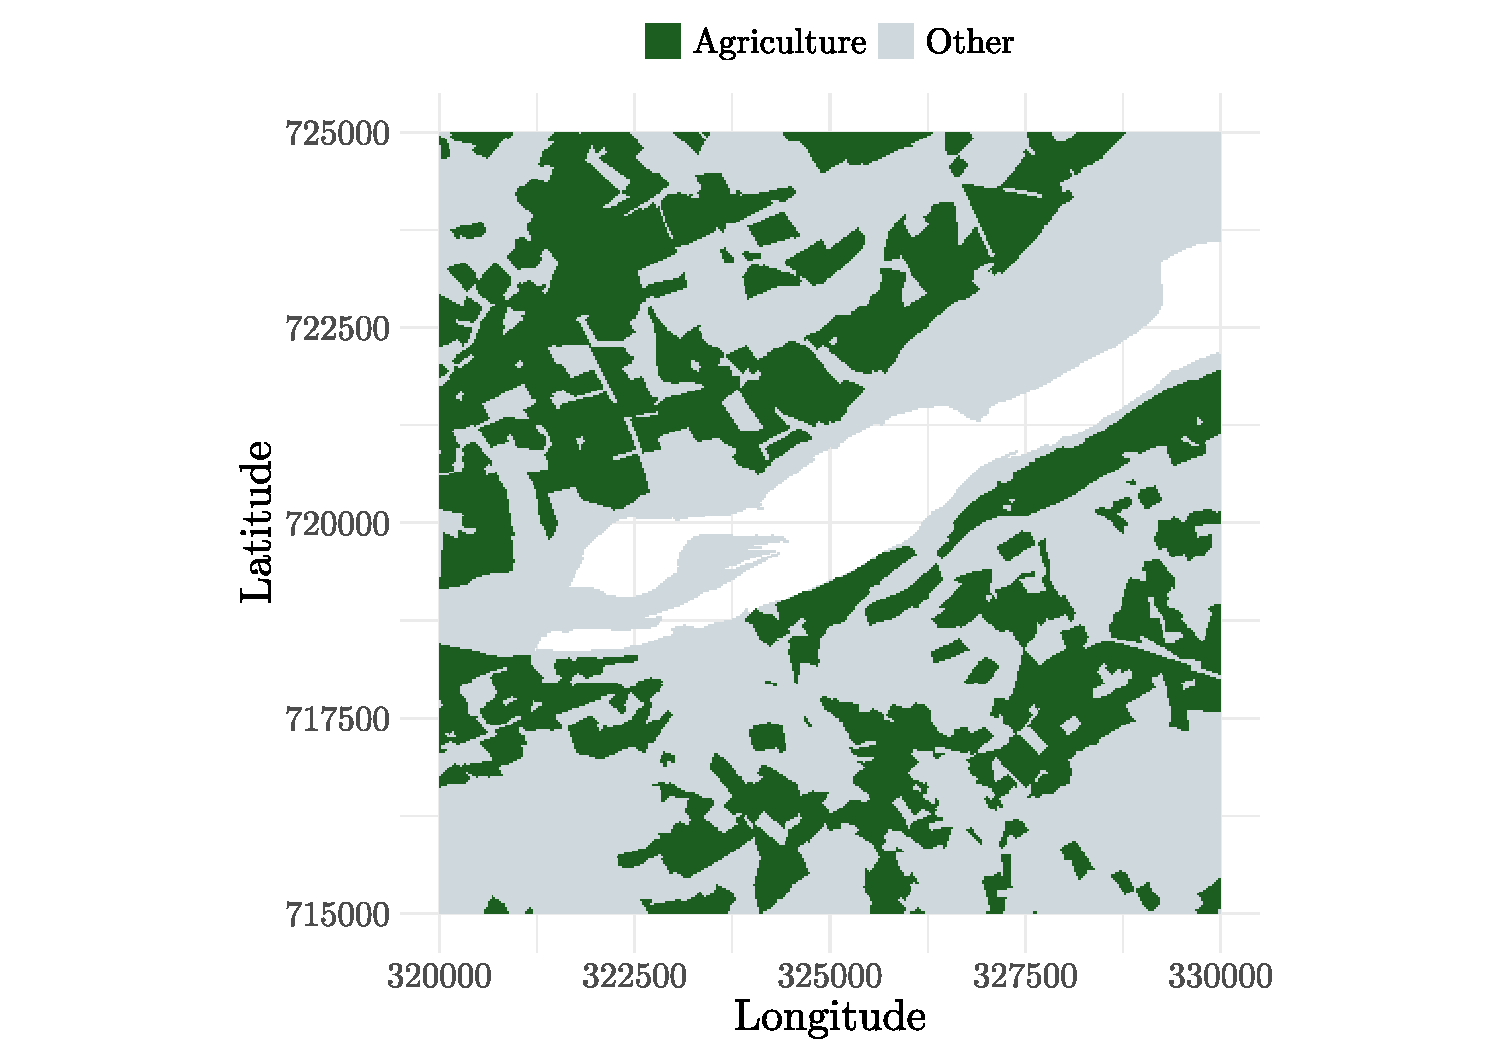
\includegraphics[width=\linewidth]{output/figures/lcm_example_area.pdf}
        \label{fig:ukceh-lcm-raw}    
    \end{subfigure}
    \begin{subfigure}{0.49\linewidth}
        \caption{\centering Agricultural raster aggregated to 1km$^2$ landscape grid cells}    
        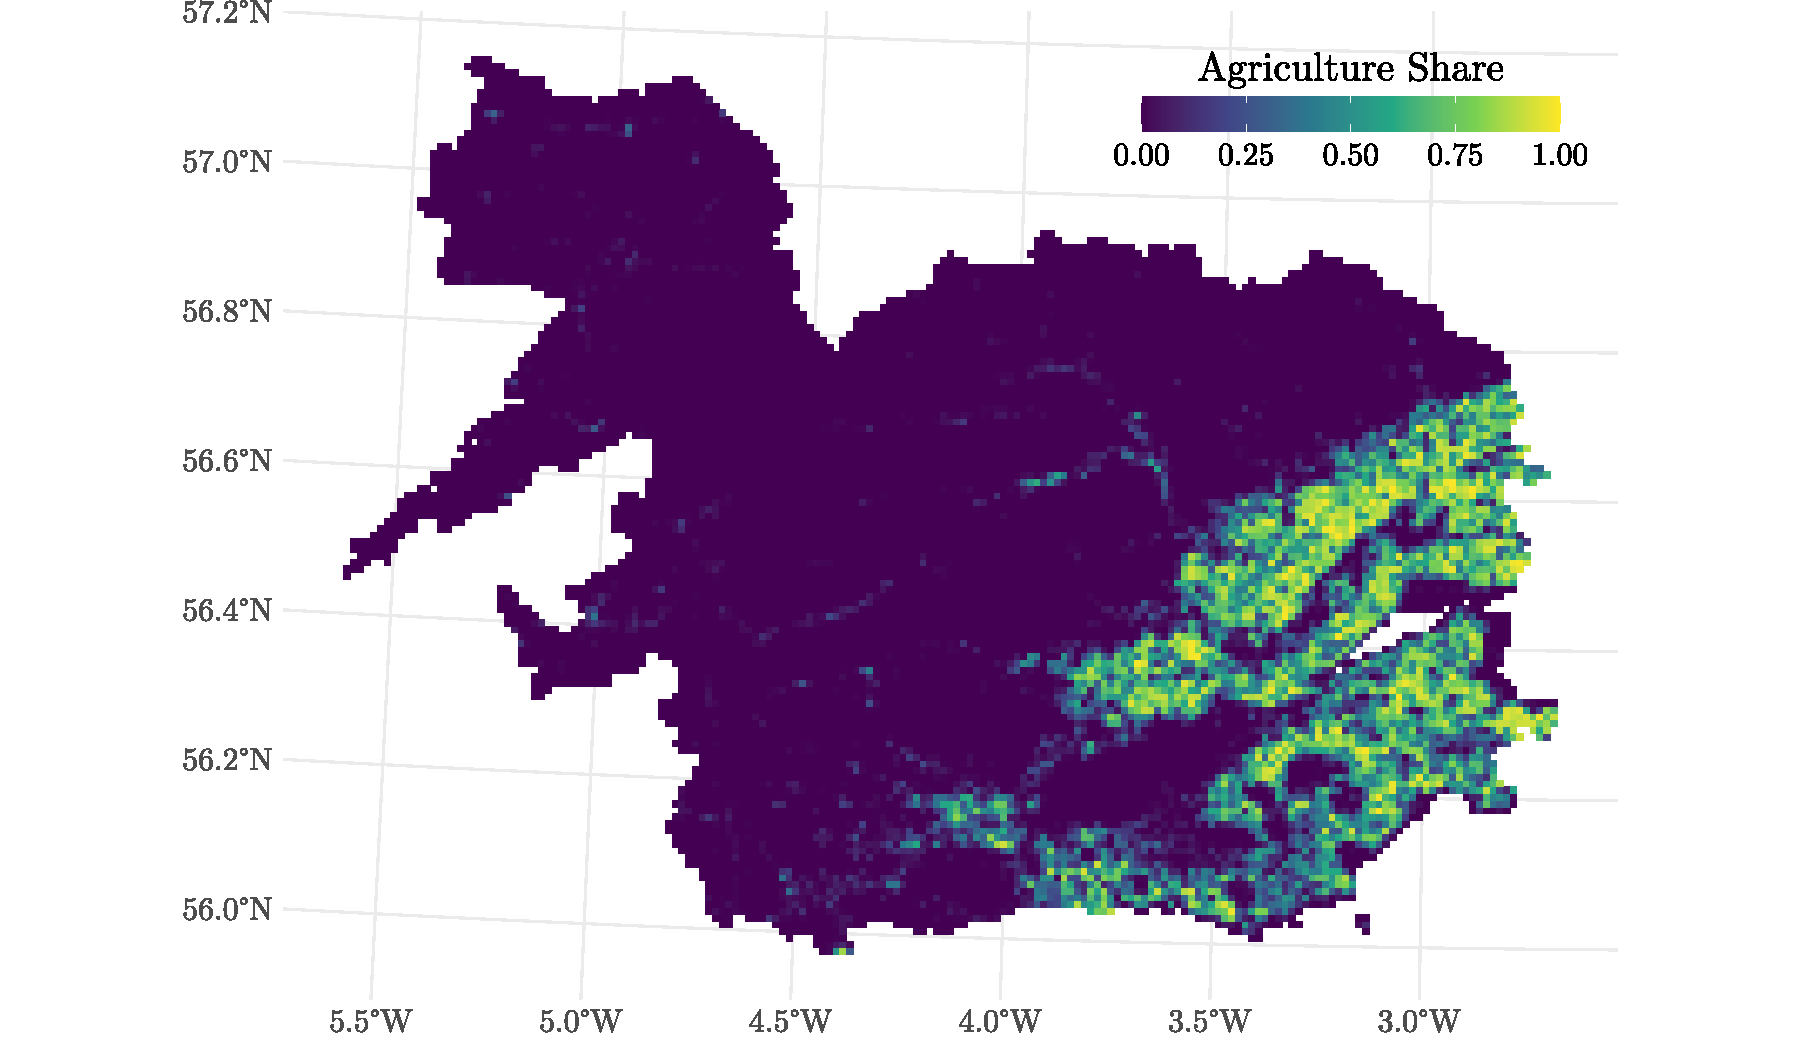
\includegraphics[width=\linewidth]{output/figures/lcm_agg_river_grid.pdf}
        \label{fig:ukceh-lcm-agg}
    \end{subfigure}
    \caption*{\justifying \footnotesize Notes: Data from the UK Center for Ecology \& Hydrology Land Cover Map (25m rasterized land parcels, GB). Fig. \ref{fig:ukceh-lcm-raw} shows the extracted agricultural layer in a subregion around the Firth of Tay. Fig. \ref{fig:ukceh-lcm-agg} includes the entire study region. 2022 data is used for illustration. See main text for details.}
\end{figure}

\subsection{Hydrometry}
To detect beaver impacts on their immediate surrounding, I obtain data on river characteristics. The Scottish Environmental Protection Agency (SEPA) operates a nationwide network of in-situ hydrometry monitoring stations, 167 of which reside in the study region. Stations collect data on rainfall, groundwater levels, river levels, river flow (or discharge), and tidal level. I extract historical records of river level, groundwater level, and river flow--all of which may be altered by beaver colonization. I drop groundwater level from analysis due to high missingness. I aggregate river level (recorded monthly) and river flow (recorded daily) to annual statistics to match the temporal resolution of the beaver expansion data.

\subsection{Soil}

\begin{figure}
    \centering
    \caption{Soil agriculture capability classes}
    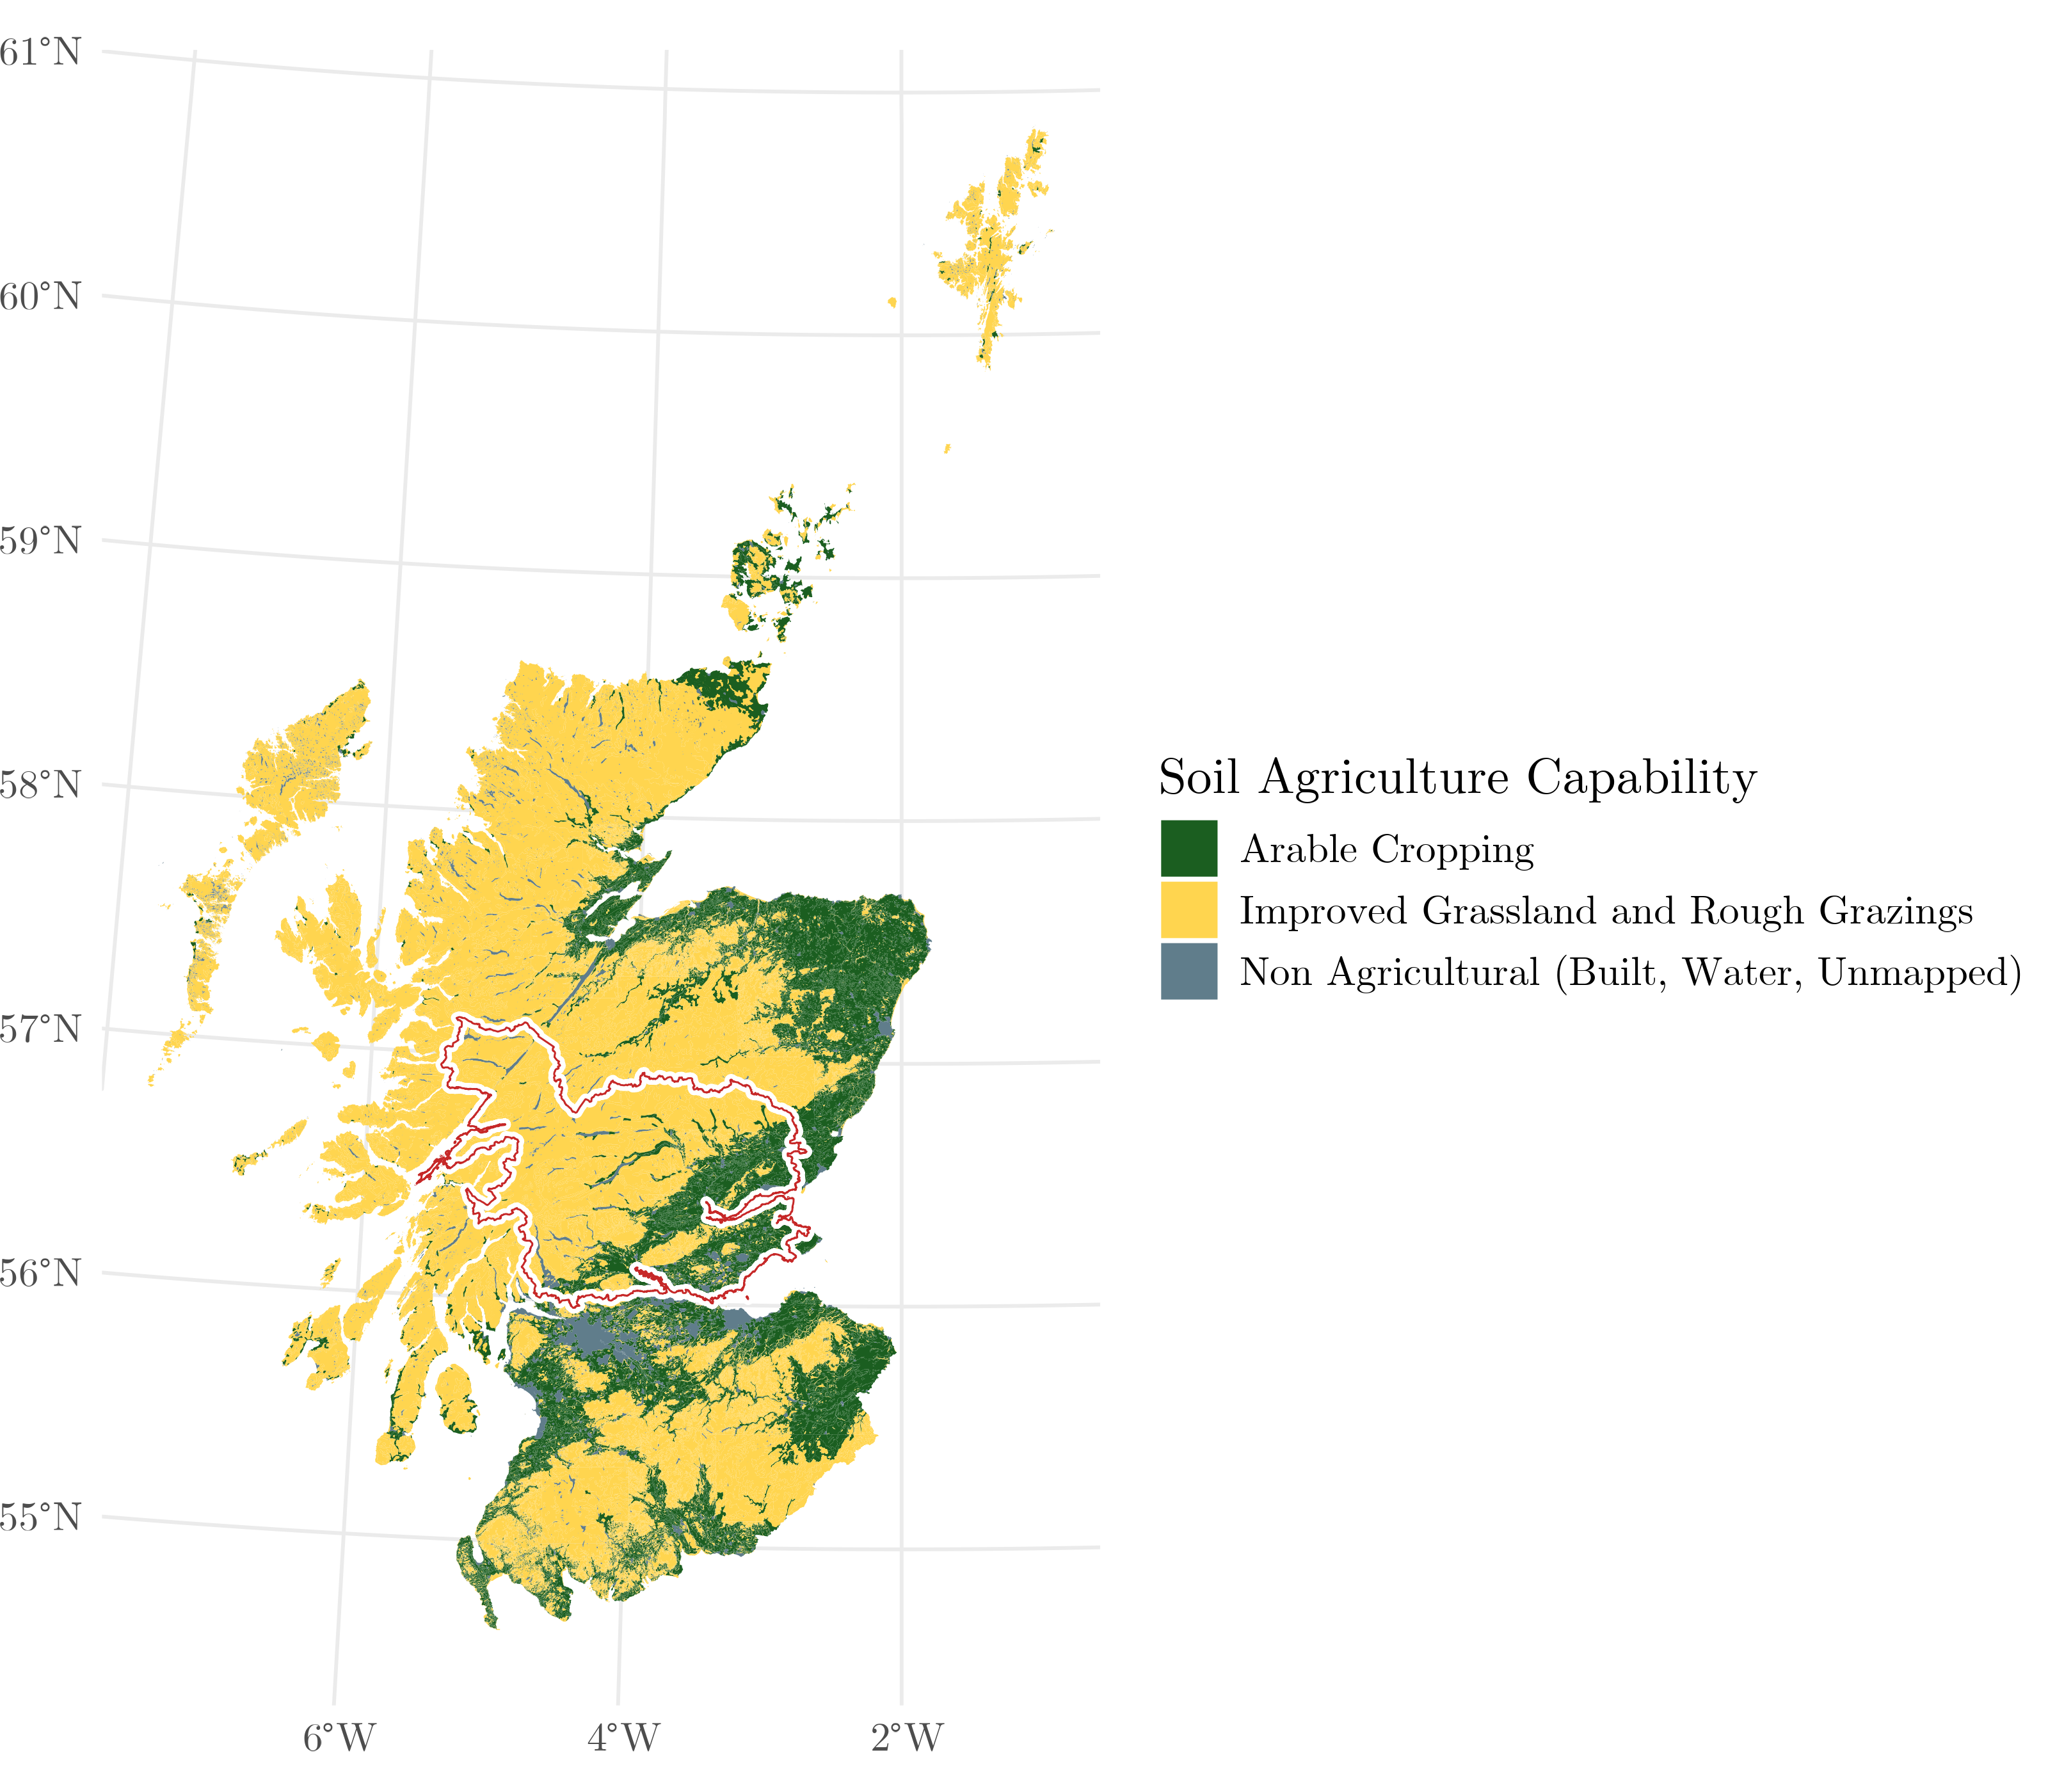
\includegraphics[width=0.6\linewidth]{output/figures/soil_lca_map.png}
    \caption*{\justifying \footnotesize Notes: Data from James Hutton Institute. Classes have been aggregated from the 13 original classifications. Study region outlined in red.}
    \label{fig:soil-lca-map}
\end{figure}

% \begin{itemize}
%     \item Elevation from ASTER (https://lpdaac.usgs.gov/products/astgtmv003/). Slope calculated as first derivative of elevation (constant)
% \end{itemize}

To distinguish between high and low agriculture-propensity areas, I use soil data from the James Hutton Institute. The soil map bins Scottish land into 13 main soil classes, ranging from soil suitable for a broad array of crops\footnote{This highest cropping suitability category is characterized by ``well-drained deep loam, sandy loams, silty loams or their related humic variants with good reserves of moisture. Sites are level or gently sloping and the climate is favourable. There are no or only very minor physical limitations affecting agricultural use'' (cite)} to soil that could be used only for rough grazing (e.g., rugged or extremely wet terrain). An additional three classes capture built, water, and unmapped island areas. In Fig. \ref{fig:soil-lca-map}, I group the 13 bins into three broad classes: Arable Cropping, Improved Grassland and Rough Grazings, and Non-Agricultural (including built, water, and unmapped areas). To achieve full cover, I employ two versions of the soil map: a 1:50,000 scale map that is considered definitive where coverage exists (mainly in eastern lowlands, where arable land is widespread) and a 1:250,000 scale map that provides lower resolution coverage in highlands areas not mapped by the 50k scale map. I calculate the share of each landscape grid cell that is occupied by a given class and determine the dominant class (>50\%) in each cell.

\subsection{Weather}

To control for variation in weather patterns across the study region, I extract temperature, precipitation, and vegetation cover records from the European Centre for Medium-Range Weather Forecasts' Reanalysis v5 (ERA5), a weather reanalysis product that provides hourly estimates at the resolution of a 31km global grid, spanning 1950 to present \citep{hersbach_era5_2020}. Using data from 1990 to 2022, I calculate annual total precipitation, average temperature at two meters, and average leaf area index. I then assign ERA5 annual grid cell values to 1km$^2$ landscape grid cells intersecting the ERA5 cell, weighting by overlap proportion when multiple ERA5 cells intersect with a single landscape cell.

% \subsection{Remote Sensing of Floods}